\section{Example}
In this example (\textit{figure \ref{fig:mapreduce_example}}), a simple word count will be performed: given a source of text, the algorithm will count the occurrences of every word appearing in such text.

\begin{figure}[H]
    \centering
    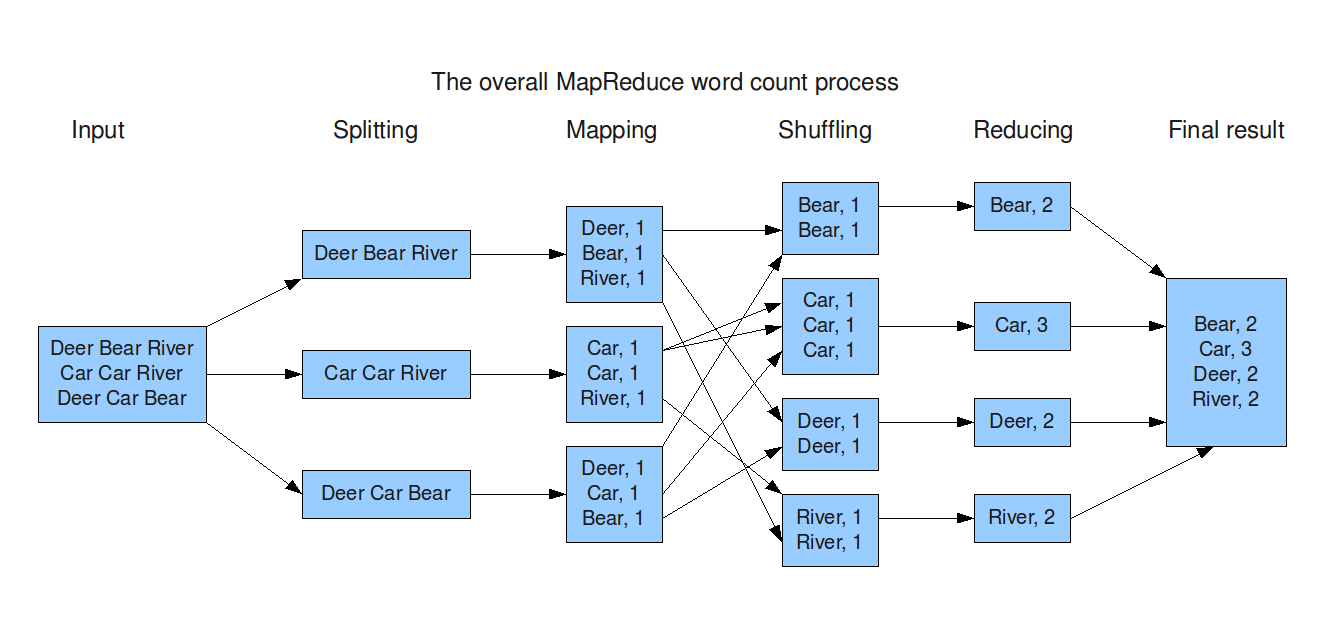
\includegraphics[width=\linewidth]{document/chapters/chapter_4/images/mapreduce_example.png}
    \caption{Example of word count expressed through the MapReduce paradigm \cite{mapreduce_example_site}}
    \label{fig:mapreduce_example}
\end{figure}

The process begins with splitting the input in smaller portions, in this case the text is split by row. On the resulting portions, the Map function is performed; in this example, every word (that is used as a key) is mapped to the value "1" (since it is one appearance of said word). The results are then grouped through the Shuffling operation, using the key as the grouping criteria. Finally, the Reduce function is executed, in different machines, on every group (the example sums the values in order to get the final number of occurrences for every word); the results of the Reduce operations is then collected, obtaining the final collection of key/value pairs.